%% CS 2883R proposal, revised from the teammate's supplied first draft.
%% Original preserved verbatim in drafts/teammate-original.tex.
%% Revision: technical clarification, controls, prose, citations, adapted TikZ.
%% Sources inspected:
%% qqgjyx/overleaf_DriftNeRF @ 79946b56b0b951b03da3b58f4ea7062e4076bfa2
%% Q9gJYx/DriftNeRF @ e7fe12f260281e0748f42b5a70fb842be0bb8af2
%% arXiv:2610.29106v1, Sections 3.3--3.4 and Appendix D.
%% Build here: latexmk -pdf -interaction=nonstopmode main.tex
\documentclass[sigconf,nonacm]{acmart}
\setcopyright{none}
\settopmatter{printacmref=false,printfolios=true}
\usepackage{tikz}
\usetikzlibrary{arrows.meta,calc,positioning}
\usepackage{graphicx}
\usepackage[capitalise,noabbrev]{cleveref}
% Notation used in the proposal and adapted schematic.
\newcommand{\vx}{\boldsymbol{x}}
\newcommand{\sg}{\operatorname{sg}}


\begin{document}
\title{Sampling Dependence in DriftNeRF's Density Consensus}
\subtitle{CS 2883R: Final Project Proposal, Fall 2026}
\author{Juntang Wang}
\affiliation{\institution{Harvard University}\city{Cambridge}\country{USA}}
\email{juntangwang@g.harvard.edu}
\author{Ciro Zhang}
\affiliation{\institution{Harvard University}\city{Cambridge}\country{USA}}
\email{cirozhang@g.harvard.edu}
\renewcommand{\shortauthors}{Wang and Zhang}
% Adapted from DriftNeRF's images/fig-overview.tex: ray/sample geometry,
% contrasting anchor/candidate colors, proximity links, rounded consensus box.
% https://github.com/qqgjyx/overleaf_DriftNeRF/blob/79946b56b0b951b03da3b58f4ea7062e4076bfa2/images/fig-overview.tex
% Citation: Wang et al., arXiv:2610.29106v1 (CC BY 4.0).
% Changes: compact two-panel layout, input-ray labels, equal candidate counts,
% stratified off-ray queries, explicit detached targets. No result data.
% Blank lines are commented because acmart collects teaser content as an argument.
\begin{teaserfigure}
\centering
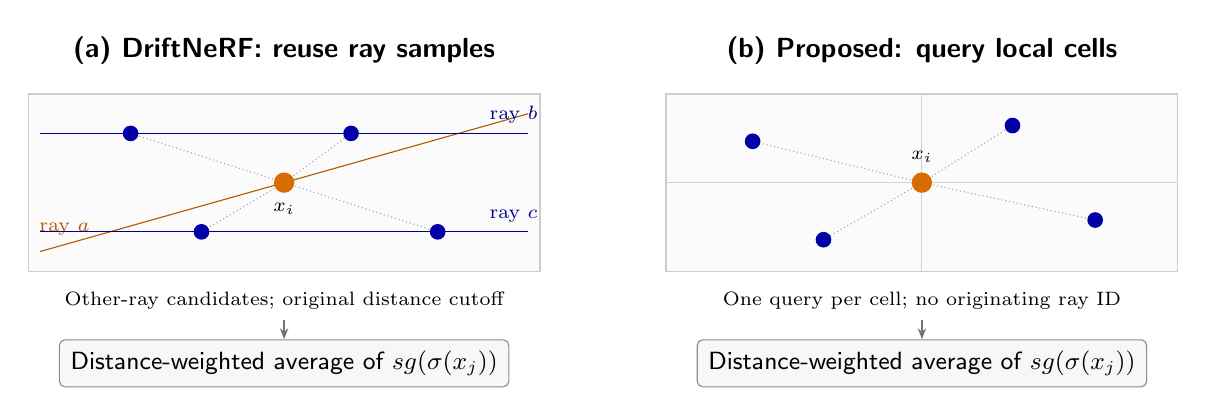
\begin{tikzpicture}[
  x=1cm,y=1cm,font=\sffamily\small,
  candidate/.style={circle,fill=blue!65!black,inner sep=2pt},
  anchorpoint/.style={circle,fill=orange!85!black,inner sep=2.6pt},
  arr/.style={-{Stealth[length=4pt]},semithick},
  target/.style={draw=black!45,rounded corners=2pt,fill=black!3,
    minimum height=0.55cm,align=center,inner sep=4pt}
]
\begin{scope}
  \node[font=\sffamily\bfseries] at (3.45,2.8)
    {(a) DriftNeRF: reuse ray samples};
  \draw[gray!40,fill=gray!3] (0.2,0) rectangle (6.7,2.25);
  \draw[orange!70!black,thin] (0.35,0.25) -- (6.55,2.0)
    node[pos=0.05,above,font=\scriptsize] {ray $a$};
  \draw[blue!55!black,thin] (0.35,1.75) -- (6.55,1.75)
    node[pos=0.97,above,font=\scriptsize] {ray $b$};
  \draw[blue!55!black,thin] (0.35,0.5) -- (6.55,0.5)
    node[pos=0.97,above,font=\scriptsize] {ray $c$};
  \coordinate (a) at (3.45,1.125);
  \foreach \x/\y in {1.5/1.75,4.3/1.75,2.4/0.5,5.4/0.5}{
    \draw[black!35,densely dotted] (a) -- (\x,\y);
    \node[candidate] at (\x,\y) {};
  }
  \node[anchorpoint,label={[font=\scriptsize]below:$\vx_i$}] at (a) {};
  \node[font=\scriptsize,align=center] at (3.45,-0.38)
    {Other-ray candidates; original distance cutoff};
  \node[target] (leftTarget) at (3.45,-1.17)
    {Distance-weighted average of $\sg(\sigma(\vx_j))$};
  \draw[arr,black!55] (3.45,-0.62) -- (leftTarget.north);
\end{scope}
\begin{scope}[xshift=8.1cm]
  \node[font=\sffamily\bfseries] at (3.45,2.8)
    {(b) Proposed: query local cells};
  \draw[gray!40,fill=gray!3] (0.2,0) rectangle (6.7,2.25);
  \draw[gray!35] (3.45,0) -- (3.45,2.25);
  \draw[gray!35] (0.2,1.125) -- (6.7,1.125);
  \coordinate (a) at (3.45,1.125);
  \foreach \x/\y in {1.3/1.65,4.6/1.85,2.2/0.4,5.65/0.65}{
    \draw[black!35,densely dotted] (a) -- (\x,\y);
    \node[candidate] at (\x,\y) {};
  }
  \node[anchorpoint,label={[font=\scriptsize]above:$\vx_i$}] at (a) {};
  \node[font=\scriptsize,align=center] at (3.45,-0.38)
    {One query per cell; no originating ray ID};
  \node[target] (rightTarget) at (3.45,-1.17)
    {Distance-weighted average of $\sg(\sigma(\vx_j))$};
  \draw[arr,black!55] (3.45,-0.62) -- (rightTarget.north);
\end{scope}
\end{tikzpicture}
\caption{Sampling constructions, adapted from DriftNeRF~\citep{wang2026driftnerf}. Orange denotes the anchor; blue denotes four candidates per panel. Dotted links connect candidates to the anchor for distance-weighted averaging. This conceptual 2D slice illustrates 3D sampling; equal displayed counts do not imply equal query costs.}
\label{fig:sampling-hypothesis}
\Description{Two panels with equal candidate counts. Left: an anchor on input ray a pools four candidate densities from other input rays b and c. Right: an anchor queries one candidate in each of four local cells, with no ray identifiers. Dotted proximity links lead to a distance-weighted detached-density target in each panel.}
\end{teaserfigure}

\maketitle
\raggedbottom
\balance

%% =================================================================
%% Research goal and problem statement
%% =================================================================
\section{Research goal and problem statement}\label{sec:goal}

Reconstructing a 3D scene from only a few images is underconstrained: different geometric configurations can reproduce the observed views. A neural radiance field (NeRF)~\citep{mildenhall2020nerf} can therefore fit its training images while producing floating artifacts or incorrect geometry from new viewpoints. Improving reconstruction with limited observations matters when dense image capture is impractical.

DriftNeRF~\citep{wang2026driftnerf} addresses this problem by pulling each anchor's density toward a distance-weighted average of nearby predictions from other rays. Its candidates come from existing renderer samples. Uniform selection from this pool does not imply uniform coverage of the underlying 3D neighborhood: camera coverage and ray sampling determine which locations can contribute to the average.

This project asks: \emph{at a fixed local query budget, does spatial stratification reduce consensus-target variability, and does that translate into better novel-view synthesis while preserving thin structures?} We propose dividing each anchor's neighborhood into equal-volume cells and querying one point per cell, as illustrated in \cref{fig:sampling-hypothesis}. Our hypothesis is that more even coverage can limit the influence of concentrated samples. The competing possibility is that surface-focused sampling provides useful guidance that off-ray queries dilute.

We will use a small subset of NeRF-Synthetic, with known camera poses and three training views per scene. Our intended contribution is an analysis of target stability on a frozen field, followed by an evaluation of reconstruction quality and computational cost during training. The main challenges are separating sampling effects from changes in the learned geometry, preserving thin structures, and keeping additional density queries affordable.

%% =================================================================
%% Relationship to prior work
%% =================================================================
\section{Relationship to prior work}\label{sec:related}

NeRF~\citep{mildenhall2020nerf} provides the field representation and rendering objective. FreeNeRF~\citep{yang2023freenerf} progressively exposes positional-encoding frequencies and penalizes near-camera density. RegNeRF~\citep{niemeyer2022regnerf} regularizes geometry and appearance in patches rendered from unobserved viewpoints and anneals its sampling space during training. Our investigation concerns sampling for an auxiliary density-consensus target, complementing work on field complexity and sampling for rendered views.

We build on DriftNeRF~\citep{wang2026driftnerf}, coauthored by Juntang Wang, and retain its field representation, detached-target update, and warmup schedule. The question we investigate is whether replacing renderer-derived candidates with spatially stratified local queries changes the stability and usefulness of the density target. This is an extension of the existing consensus construction; the new work is the sampling analysis and its controlled comparison with independent uniform local queries.

%% =================================================================
%% Proposed investigation
%% =================================================================
\clearpage
\section{Proposed investigation}\label{sec:method}

\paragraph{Consensus construction.}
DriftNeRF draws anchors and a shared candidate pool uniformly without replacement from the renderer's samples. For anchor position $\vx_i$, let $C_i$ be the candidate set, $\sigma(\vx)$ the predicted density, and $d_{ij}=\|\vx_i-\vx_j\|_2$ the distance to candidate $j$. The target is
\begin{equation}
\label{eq:consensus}
\begin{aligned}
\bar\sigma_i &= \frac{\sum_{j\in C_i} w_{ij}\,\sg\!\left(\sigma(\vx_j)\right)}{\sum_{j\in C_i}w_{ij}},\\
w_{ij} &= m_{ij}\exp(-d_{ij}/\tau).
\end{aligned}
\end{equation}
Here $\sg$ denotes stop-gradient, $\tau>0$ sets the decay scale, and $m_{ij}$ is an eligibility indicator. In DriftNeRF, $m_{ij}=1$ only for different-ray pairs with $d_{ij}\leq d_{\max}$, where $d_{\max}$ is the cutoff. Anchors with a zero denominator are excluded. Detaching candidate densities in \cref{eq:consensus} directs the auxiliary gradient through the anchor branch.

\paragraph{Diagnosis.}
We will first freeze a trained field and fix the anchors and renderer sample pool. Repeated candidate draws will measure within-scheme target variability and shifts in the mean target between sampling schemes. We will also record the fraction of anchors with eligible neighbors and, for valid anchors, effective neighbor counts: squared total weight divided by the sum of squared weights. These diagnostics describe target construction; higher coverage or lower variability alone does not establish better geometry.

\paragraph{Stratified local queries.}
We propose dividing a cube centered on each anchor into equal-volume cells and drawing one point uniformly within each cell. The cube will lie within the distance cutoff. We will query the existing NeRF at these locations and use the same exponential kernel and detached-target construction. For these points, $m_{ij}=1$ because eligibility is spatial; they have no originating camera-ray identifiers. This changes cross-ray consensus into a local field regularizer and requires new density evaluations, but no additional images or depth information.

The primary control will draw independent uniform points in the same cube. In the frozen-field diagnostic, both off-ray variants will share the field, anchors, cube size, kernel scale, and number of queries per anchor, isolating stratification. We will also compare with the original renderer-pool construction. That comparison changes the averaging support and ray eligibility as well as sample placement, so it tests the combined effect of the extension.

\paragraph{Training and evaluation.}
We will compare vanilla NeRF, original DriftNeRF, and both off-ray variants using matched input views, initialization seeds, architecture, and training steps. Each regularized variant retains the photometric loss and adds the mean squared difference between anchor density and its detached target. As in DriftNeRF, the penalty weight rises linearly during the first 10\% of training. We will use a shared regularization weight for the primary comparison and examine a few neighborhood sizes, query counts, and penalty strengths as sensitivity checks.

We will report PSNR, SSIM, and LPIPS on held-out views, summarize variation across matched seeds, and inspect floaters and thin structures. We will measure elapsed training time and total density-query counts: DriftNeRF reuses a pool shared across anchors, whereas the extension makes new queries per anchor. Equal candidate counts therefore do not imply equal computation. Test views will be reserved for final evaluation rather than parameter selection.

The extension will be useful if its quality gains are repeatable and justify the measured cost without degrading thin structures. Lower target variability without better rendering, excessive query cost, or loss of thin structures will instead identify limits of the proposed sampling strategy.

%% =================================================================
%% AI usage acknowledgement
%% =================================================================
\section*{AI usage acknowledgement}\label{sec:ai}
OpenAI Codex was used for brainstorming, technical feedback, and revisions to the structure and wording of our draft, including experimental comparisons, citations, and the TikZ schematic. No experiments were run for this proposal.
% AUTHOR REVIEW: Update this acknowledgement after your own final rewrite to
% reflect actual use. Add any other AI tool used for the first draft/schematic.
% AUTHOR REVIEW: Confirm individual contributions before the final report.

\bibliographystyle{ACM-Reference-Format}
\bibliography{ref}
\end{document}
